%%%%%%%%%%%%%%%%%%%%%%%%%%%%%%%%%%%%%%%%%%%%%%%%%%%%%%%%%%%%%%%%%%
\documentclass[article,12pt,oneside,a4paper,english,brazil,sumario=tradicional]{abntex2}		
% Pacotes usados
%\usepackage{times}%Usa a fonte Latin Modern
\usepackage[T1]{fontenc}%Selecao de codigos de fonte.
\usepackage[utf8]{inputenc}%Codificacao do documento
\usepackage{indentfirst}%Indenta o primeiro parágrafo de cada seção.
\usepackage{float}
\usepackage{nomencl}%Lista de simbolos
\usepackage{color}%Controle das cores
\usepackage{graphicx}%Inclusão de gráficos
\usepackage{microtype}%Para melhorias de justificação
\usepackage{setspace}
\usepackage{lipsum}%Para geração de dummy text
\usepackage{ragged2e}
\usepackage[abnt-emphasize=bf,abnt-and-type=e,alf]{abntex2cite}%Citações ABNT
\usepackage{mathptmx}
%\usepackage[bottom=2cm,top=3cm,left=3cm,right=2cm]{geometry}
\usepackage{bookman}
\usepackage{enumitem}
\usepackage{enumerate}

\usepackage{times}
\usepackage{amsmath}
\usepackage{amssymb}
\usepackage{mathtools}
\usepackage{geometry}


% Configuracoes do documento
\graphicspath{{./Figuras/}}%Images na pasta "Figuras"
\setsecheadstyle{\bfseries \large \uppercase}
%\setsubsecheadstyle{\normalsize \uppercase}
\setsubsubsecheadstyle{\bfseries \normalsize }
\setlrmarginsandblock{2.5cm}{2.5cm}{*}%Margens esquerda-direita
\setulmarginsandblock{4cm}{2.5cm}{*}%Margens cima-baixo
\checkandfixthelayout
\setlength{\parindent}{1.0cm}%paragrafo
%\doublespacing %espacamento de 2
%\setlength{\ABNTEXcitacaorecuo}{4cm}%recuo citacao direta +3

\begin{document}
\selectlanguage{brazil} % Seleciona o idioma do documento
\frenchspacing % Retira espaço extra obsoleto entre as frases.

\begin{center}
%TITULO
    \SingleSpacing
	\uppercase{\bfseries{\Large{Utilização e comparação entre métodos de Sintonia para Controlador PID aplicados à planta de um complexo Biomecânico Canela-pé}}}
	\vspace{12pt}
	\\
\end{center}

\begin{center}
    %AUTOR - Pode-se contar com infinitos autores   :)
	\normalsize{AZEVEDO,N.S.$^1$;MENEZES,L. L.$^1$;RAZONI, R. R.$^1$; SAMPAIO, M.R.C.$^1$; TELES, J.V. de J.$^1$}
	\begin{center}
	\SingleSpacing{
	\normalsize{$^1$Universidade Salvador,Faculdade de Engenharia, Arquitetura e TI, Departamento de Engenharia Elétrica. E-mail para contato: naiaraazevedo62@gmail.com;
	lucasluis14@hotmail.com;
	ranerazoni@hotmmail.com;
	samppaiomari@gmail.com;
	joaotb14@gmail.com
	}}

	\end{center}


\end{center}

\begin{flushleft}
\begin{SingleSpace}
\RaggedRight
\noindent
\small{RESUMO-}
\noindent
\normalsize{\textit{O objetivo deste trabalho é demonstrar a sintonização de um controlador PID utilizando quatro métodos de sintonia diferentes. Foi utilizado um sistema baseado
na planta de uma perna mecânica para paraplérgicos, a qual apresenta uma função de transferência de ordem superior proveniente do seu sistema de controle. Os métodos escolhidos para a sintonização foram o segundo método de Ziegler Nichols, o método IMC, o método de Tyreus e Luyben e o método de aproximações sucessivas. Após a aplicação e análise dos resultados destas sintonias foram realizadas comparações entre os diferentes resultados e concluiu-se que o método mais eficiente foi o de Aproximações sucessivas. A execução de todos os algoritmos foi feita utilizando o software MATLAB.}}

\end{SingleSpace}

%TEXTO DO RESUMO (em português}


%\noindent
%PALAVRAS-CHAVE} 
%\textbf{Palavras-chave}: PC1, PC2, PC3 e PC4.
\end{flushleft}

\textual
\pagestyle{simple}
\pagenumbering{arabic}
%\aliaspagestyle{chapter}{simple}


\section{\large Introdu\c c\~ao}
\label{secIntroducao}
\normalsize
\SingleSpacing
Com os avanços da automação na indústria e no dia-a-dia da sociedade, o controle vem se tornando uma área de intensa pesquisa, expandindo-se a inúmeras opções de aplicabilidade.
As características mais importantes no momento de se definir um controlador é a sua robustez, estabilidade e desempenho eficiente, assim, os controladores PID destacam-se no momento da escolha, principalmente em processos industriais.  

Em tal controlador os parâmetros proporcional, integral e derivativo devem ser ajustados de acordo com o processo de aplicação. Tais ajustes devem ser realizados da maneira mais adequada possível para que não se obtenham respostas indesejadas, assim torna-se essencial a escolha de uma boa sintonização do sistema de controle. Uma das primeiras técnicas de sintonia propostas foi a de Ziegler-Nichols \cite{zn} na
tentativa de obter melhores ajustes para os parâmetros do controlador a partir das suas tabelas indicadas. 

Cada um dos métodos de sintonia existentes é otimizado em função de um determinado aspecto do sistema, assim, cada um deles tem suas vantagens e limitações, cabendo ao projetista decidir qual se encaixará da melhor maneira no controle desejado. Com o propósito de identificar um método de sintonia adequado para obter a estabilidade de um sistema biomecânico ( figura \ref{canela})com uma função de transferência de ordem superior (grau 3) testamos e comparamos quatro métodos de sintonia ao longo deste artigo, escolhendo enfim, a melhor sintonização do referenciado processo, a partir do critério de tempo de estabilização e suavidade da curva sintonizada, garantindo um maior conforto e praticidade ao paciente.
\begin{figure}[H]
    \centering
    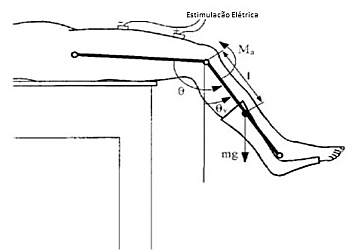
\includegraphics[scale=0.5]{canneal.png}
    \caption{Sistema Biomecânico de um complexo Canela-pé. }
    \label{canela}
\end{figure}


\section{\large Metodologia}
\SingleSpacing

O modelo a ser utilizado foi baseado na monografia de \cite{lovoestudo}, onde a planta a ser controlada é um
modelo baseado na reanimação dos músculos inferiores a partir de estímulos elétricos, utilizando o controle a fim de elevar a perna do estado de repouso até um ângulo específico e fazendo-a retornar à posição inicial (pela ação da gravidade) com a retirada da estimulação no músculo de maneira eficiente, prática e sem gerar danos ao paciente.

O modelo matemático foi proposto por por \citeonline{ferrarin} e relaciona a largura de pulso aplicada ao músculo do membro inferior com o torque gerado em torno da articulação
do joelho, considerando a coxa (fixa) e o complexo canela-pé como rígidos enquanto o tornozelo foi retirado do modelo a fim de simplificar o sistema de controle. A partir da função de transferência gerada por \cite{lovoestudo}, que relaciona o ângulo da canela com o torque
ativo do joelho devido à estimulação elétrica, linearizada e mostrada na equação \ref{mod} estudamos quatro métodos de sintonia e aplicamos a fim de comparar os seus resultados e eficiência.

\begin{equation}
    G(s) =\frac{42500}{0,3443s^3+0,6188s^2+7,842s+7,962 }
    \label{mod}
\end{equation}


\section{\large Resultados e discussões}
\SingleSpacing
% TEXTO DO DESENVOLVIMENTO

\subsection{\large Método de Sintonia de Ziegler Nichols}

Foi utilizado o segundo método de Ziegler Nichols adequado a um sistema de malha fechada.
Para o cálculo do período ($P_{cr}$) e ganho ($K_{cr}$) critico utilizados neste método de sintonia, aplicamos o método do relé ideal em malha fechada \cite{releas}, o qual provoca oscilações limitadas e controladas na estimação da resposta em frequência da planta. A partir da análise gráfica da saída do relé (figura \ref{rele}) na planta conseguimos identificar o valor de $P_{cr}$ e calcular o $K_{cr}$ do sistema.

\begin{figure}[H]
    \centering
    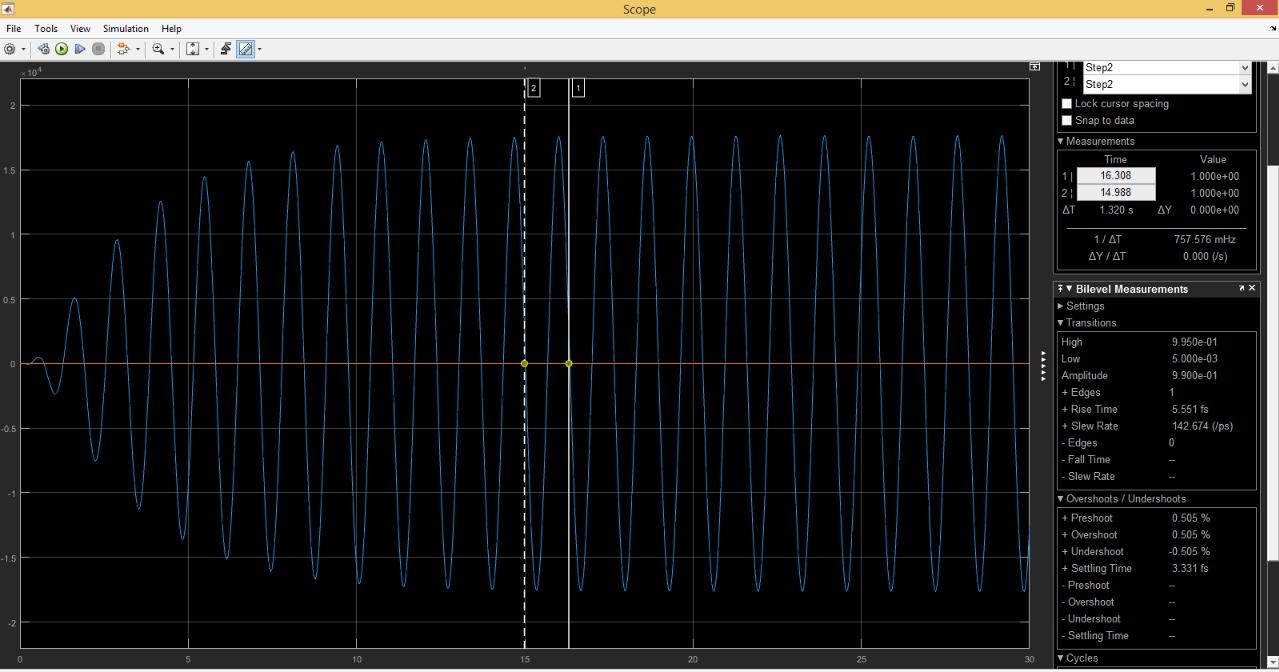
\includegraphics[scale=0.28]{rele.jpg}
    \caption{Análise gráfica da saída do relé.}
    \label{rele}
\end{figure}

Assim encontramos os valores de 1,32s para o período crítico  enquanto que para o ganho crítico o valor achado foi de 0,000144, através da equação \eqref{kcr}, utilizando $d=2$ e $a=1,76$ obtidos por análise gráfica. 
\begin{equation}
K_{cr}=\frac{4d}{\pi a}= 1,44 \times 10^{-4}
    \label{kcr}
\end{equation}
Assim calculamos os parâmetros pela tabela do segundo método de Ziegler Nichols para controle PID mostrado em \ref{ZN} e obtemos os parâmetros do controldor, indicados na mesma tabela. 

\begin{table}[H]
\centering
\caption{ Tabela para parametrização do PID a partir do segundo método de ZN.}
\begin{tabular}{|l|l|l|l|}
\hline
Tipo de Controlador  & $K_p$ & $T_i$ & $T_d$ \\\hline
PID & 0.6$K_{cr}$ & 0.5$P_{cr}$ & 0.125$P_{cr}$ \\\hline
PID (resultado) & 0.0000864 & 0.66 & 0.165\\\hline
\end{tabular}

\label{ZN}
\end{table}

Assim, após a aplicação dos valores calculados o sistema sintonizou em aproximadamente 4,24 segundos. Os tempos de sintonização apresentam um erro de mais ou menos 20$\%$. O resultado da sintonia pode ser visto na figura \ref{sintZN}.

\begin{figure}[H]
    \centering
    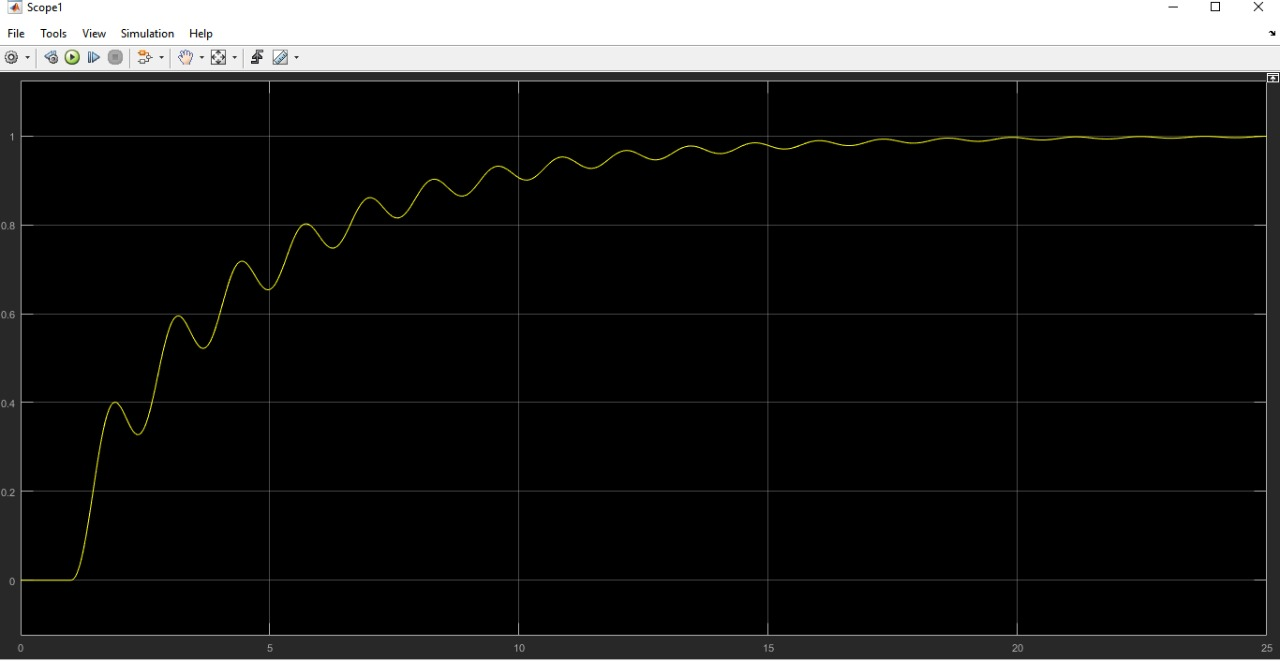
\includegraphics[scale=0.22]{zncerto.jpg}
    \caption{Resposta da malha para a sintonização pelo método de Ziegler Nichols.}
    \label{sintZN}
\end{figure}


\subsection{\large Método de Sintonia IMC}
Para aplicar esta sintonia, devido à ordem superior da nossa função de transferência, fomos levados a reduzir a mesma para uma função de segundo grau e assim encaixá-la em uma das formas mostradas na tabela de ajuste de modelos do próprio método. Analisamos a função , a partir da observação de seu gráfico de amplitude em função do tempo visto na figura \ref{func}.

\begin{figure}[H]
    \centering
    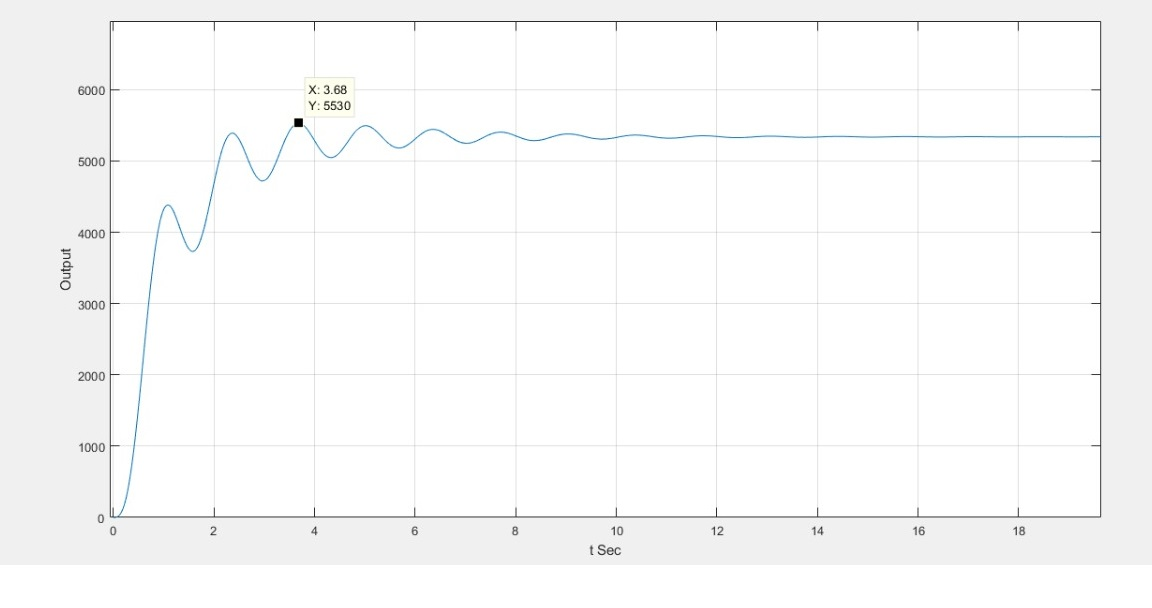
\includegraphics[scale=0.32]{func.jpg}
    \caption{Resposta da função de transferência de terceira ordem.}
    \label{func}
\end{figure}
A partir da observação gráfica encontrou-se tanto o tempo de pico, equivalente a 3,86s, quanto o máximo sobressinal da função, que resultou em um valor de 180. Assim calculou-se os parâmetros do modelo de segunda ordem, a partir das equações \ref{param} e \ref{wn}, resultando na equação característica \ref{fim} com a substituição dos parâmetros no formato adequado.
\begin{equation}
    \xi =\sqrt{\frac{{(\frac{\ln{M_p}}{\pi})}^2}{1+{(\frac{\ln{M_p}}{\pi})}^2}}=0,8556
   \label{param} 
\end{equation}

\begin{equation}
    W_{n}=\frac{\pi}{t_{p}\sqrt{1-\xi^{2}}}=1,6492
    \label{wn}
\end{equation}

\begin{equation}
G(s)=\frac{1,6942^{2}}{s^{2}+2(0,8556)(1,6492)s+ 1,6942^{2}}=\frac{2,7198}{s^{2}+2,82815+ 2,7198}
    \label{fim}
\end{equation}
   
Analisando o modelo encontrado  foi possível obter o valor referente ao $\tau$ da função. O valor encontrado foi de 0,6063s enquanto que o valor do $\lambda$ foi de 6,5961, equivalente a três vezes o valor do $\tau$. Assim a equação \ref{fim} ajustada para que ficasse equivalente ao formato mostrado na tabela \ref{imc}, a partir da conclusão de que $\xi$ equivale a 0,8556, o $K$ à 2,7198 e o $\tau$ à 0,6063. A partir do cálculo dos parâmetros pela tabela \ref{imc} teríamos os valores de $K_p$, $T_i$ e $T_d$ respectivamente de 0,0577;  1,0375 e 0,3543. 


\begin{table}[H]
\centering
\caption{ Tabela para parametrização do PID a partir do método IMC utilizando o modelo de processo indicado.}
\begin{tabular}{|l|l|l|l|}
\hline
Modelo do processo  & $K_p$ & $T_i$ & $T_d$ \\\hline
$\frac{K}{\tau^{2}s^{2}+2\tau \xi + 1} $& $\frac{2\xi \tau}{K \times \lambda}$  & $2\xi\tau$ &  $\frac{\tau}{2\xi}$ \\\hline

\end{tabular}

\label{imc}
\end{table}

Finalmente ao realizar a simulação da sintonia obtivemos uma estabilização da função em aproximadamente 4,99 s. O resultado pode ser visto na imagem \ref{imcfig}

\begin{figure}[H]
    \centering
    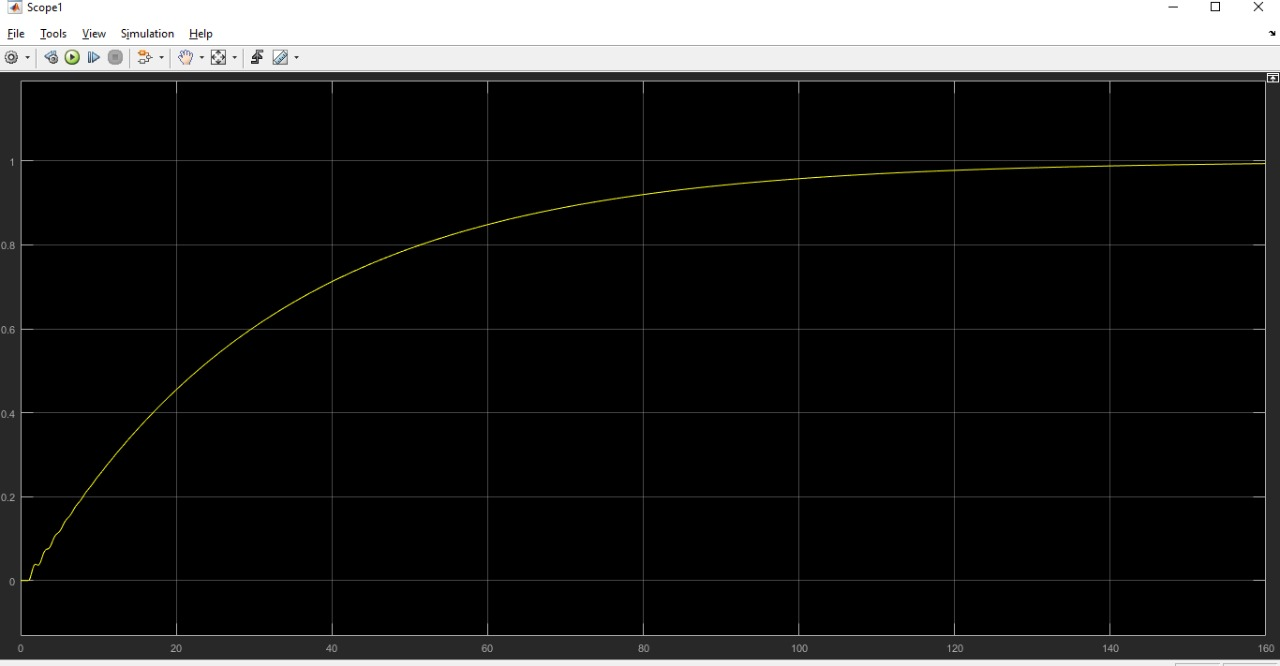
\includegraphics[scale=0.255]{imc.jpg}
    \caption{Sintonia da malha pelo método IMC.}
    \label{imcfig}
\end{figure}

\subsection{\large Método de Sintonia por Tyreus e Luyben}

A aplicação deste método baseou-se na substituição dos valores já encontrados de $K{cr}$ e $P_{cr}$ do sistema na tabela \ref{tl} para encontrar os parâmetros do controlador PID. Assim os valores encontrados de $K_p$, $T_i$ e $T_d$ foram respectivamente 0,0000654; 2,904 e 0,2094. Porém foi percebido que a sintonia poderia ser melhorada a partir do refinamento proporcional dos parâmetros a partir da alteração do valor da constante de multiplicação do Td. Os novos parâmetros são apresentados na tabela \ref{tl}.
\begin{table}[H]
\centering
\caption{ Tabela para parametrização do PID a partir do método de Tyreus e Luyben.}
\begin{tabular}{|l|l|l|l|}
\hline
Controlador  & $K_p$ & $T_i$ & $T_d$ \\\hline
PID& $0,5K_{cr}$ & $2,2 P_{cr}$ &  $0,1587 P_{cr}$ \\\hline
PID(alterado)&$0,2863 K_{cr}$ &$1,3862 P_{cr}$ & $0,1 K_{cr}$  \\\hline

\end{tabular}

\label{tl}
\end{table}

Após a reparametrização os valores encontrados de $K_p$, $T_i$ e $T_d$ foram respectivamente de  0,0000412;1,829 e 0,132. Assim foi realizada a sintonização da malha, obtendo a estabilização da função em 4,16 s. O resultado pode ser visto na figura \ref{tlfig}.

\begin{figure}[H]
    \centering
    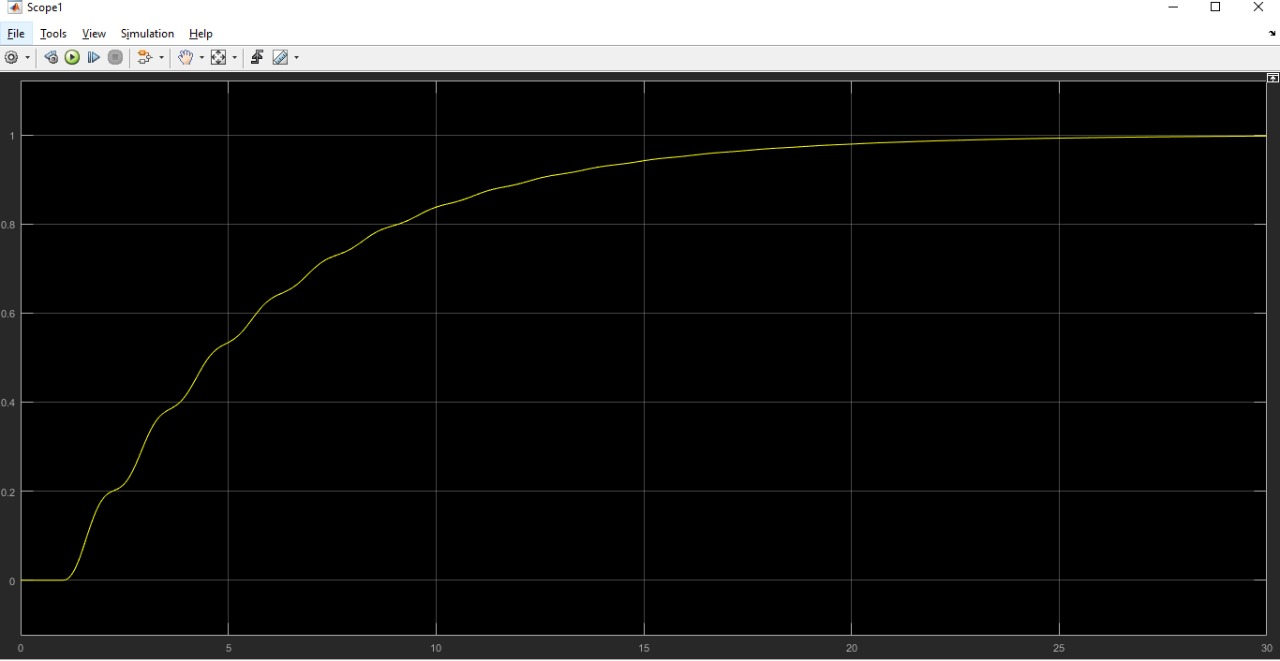
\includegraphics[scale=0.26]{tl.jpg}
    \caption{Sintonia da malha pelo método de Tyreus e Luyben.}
    \label{tlfig}
\end{figure}

\subsection{\large Método de sintonia das aproximações sucessivas ou tentativa e erro}

O último método utilizado foi o das aproximações sucessivas, que consiste em eliminar a ação integradora ($T_{i}=infinito$) e a ação derivativa ($T_{d}=0$), e aumentar $K_{p}$  até a forma de onda se tornar uma senóide. Após isso, se reduz o de $K_{p}$ pela metade. A partir daí, $T_{i}$ é reduzido aos poucos até que a curva se torne uma novamente uma senóide, e $T_{i}$ é alterado para 3x esse valor. Aumentamos $T_{d}$ aos poucos até que a curva se torne uma senóide outra vez, e ajustamos $T_{i}$ para 3x esse valor;


Assim foram encontrados os respectivos valores para $K_p$, $T_i$ e $T_d$: 0,0000007680; 130,12 e 2,2475. Os valores foram aplicados ao controlador e a sintonia encontrada pode ser observada na figura \ref{ap}.
\begin{figure}[H]
    \centering
    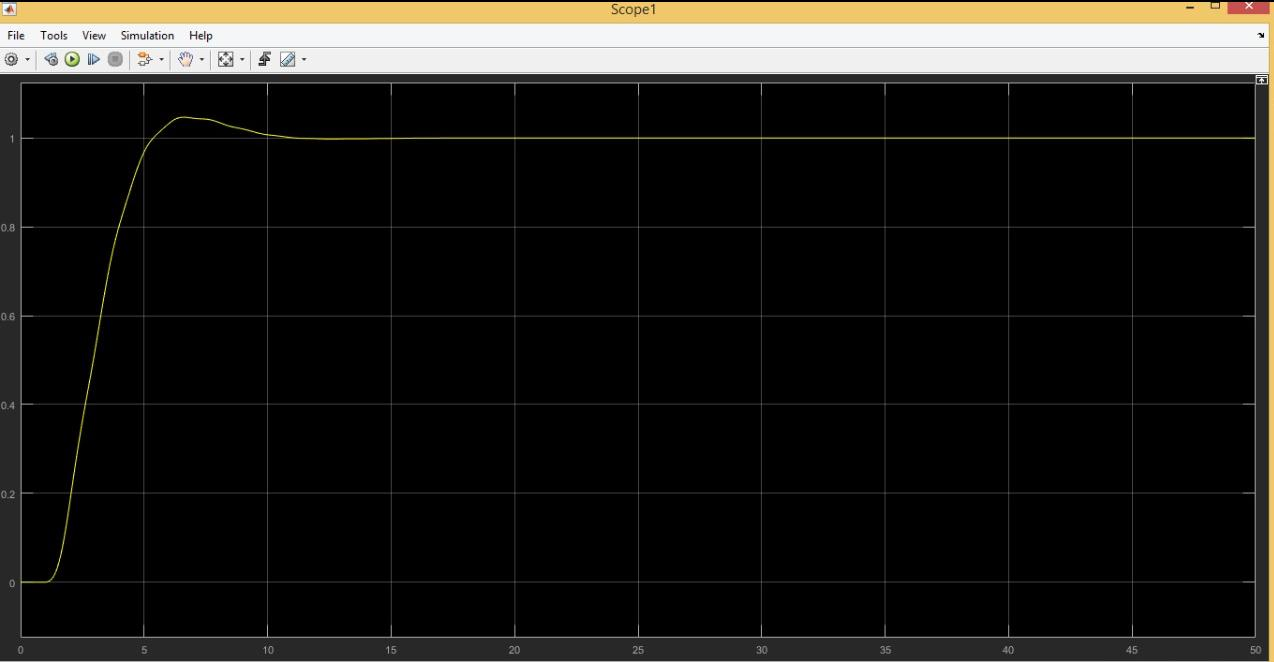
\includegraphics[scale=0.35]{ap.jpg}
    \caption{Sintonia pelo método de proximaçãoes sucessivas}
    \label{ap}
\end{figure}


\subsection{\large Comparações e índice de desempenho das sintonias}

As comparações entre os métodos foram realizadas a partir do cálculo dos índices de desempenho por um diagrama de blocos no próprio \textit{MatLab}. Os índices escolhidos foram o IAE, ITSE e o ITAE. Além da comparação entre estes, os tempos de estabilização foram também utilizados na análise para identificar a melhor sintonia.
O resultado desta comparações pode ser visto na figura \ref{comparar}, assim como o método escolhido como mais adequado ao sistema em questão, o método IMC. Apesar do método de aproximações sucessivas apresentar bons resultados, é necessário um alto conhecimento da planta em que será aplicado, para que se tenha confiança em sua eficiência.

\begin{figure}[H]
    \centering
    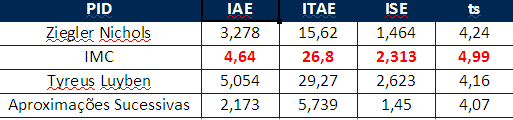
\includegraphics{comparar.png}
    \caption{Comparação entre os métodos de sintonia utilizados.}
    \label{comparar}
\end{figure}

\subsection{\large Sintonias Discretas}

Todas as sintonias vistas foram ainda convertidas para o domínio discreto e analisadas de forma eficiente, com exceção da sintonia por aproximações sucessivas. Assim, pode-se dizer que os métodos utilizados tiveram bons resultados tanto no domínio contínuo como no discreto. 

O problema do método das aproximações sucessivas no domínio discreto foi observado a partir da análise dos seus polos pelo lugar das raízes, onde concluiu-se que não seria possível sintonizar tal método no domínio discreto pois seus polos encontravam-se fora do circulo unitário. 

\subsection{\large Sintonia ótima}

Após analisarmos os parâmetros de todos os métodos chegamos a conclusão de que o método IMC atendia aos critérios estabelecidos para uma sintonia ótima, além de atender ao tempo de amortecimento desejado, equivalente ou menor que 5 segundos. Assim, tal artifício foi utilizado como nosso método de sintonia ótima. 


\section{\large {Conclusão}}
Conclui-se que existem uma variedade de métodos que podem ser utilizados para realizar a sintonia de um controle PID a depender do processo em que será empregado o controle. Neste artigo foi definido como  melhor método de sintonia o método IMC por ter atendido melhor ao critério estabelecido para a nossa planta Biomecânica, ou seja, apresentar menor tempo de estabilização e uma curva mais suave de sintonização, além de maior nível de confiança.

Conclui-se também a partir deste trabalho que o PID pode não ser o melhor controlador para o sistema em questão, mas ainda sim, se mostra eficaz a depender dos parâmetros e condições impostos pelo projetista ao controlador.



\renewcommand{\bibsection}{\section{\large {REFER\^ENCIAS BIBLIOGR\'AFICAS}}}
\bibliographystyle{abntex2-alf}
\bibliography{Referencias}
\end{document}